\section{Results}

All results are the average of the statistics captured by each node participating, and have been grouped similarity.

\subsection{Tests 1 and 2}
Test one featured the sequenced reliable (SRC) protocol in a two node configuration with a 200ms resend time, and another run with the
the unreliable protocol (SUC) with a window size of 8. The system was configured with two DGI nodes with a transient link between them.
The mean group size is presented in Figure \ref{fig:MGS-2NODE-200}, and the amount of time in group is shown in Figure \ref{fig:IGT-2NODE-200}.

\begin{figure}[!h]
\centering
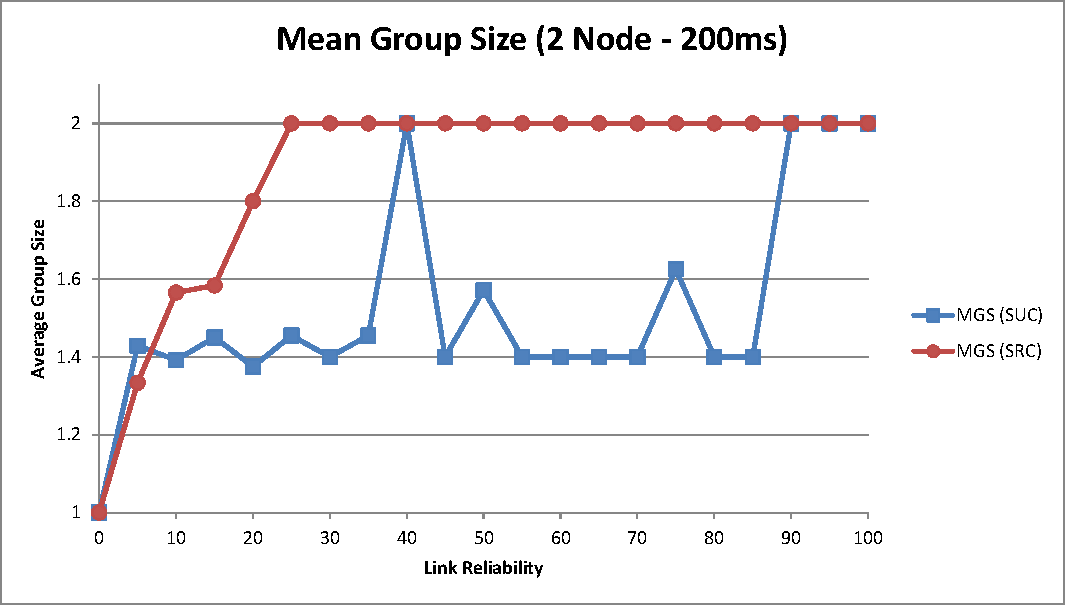
\includegraphics[width=.74\textwidth]{MGS-2NODE-200.pdf}
\caption{Average size of formed groups for two node system with 200ms resend time}
\label{fig:MGS-2NODE-200}
\end{figure}

\begin{figure}[!h]
\centering
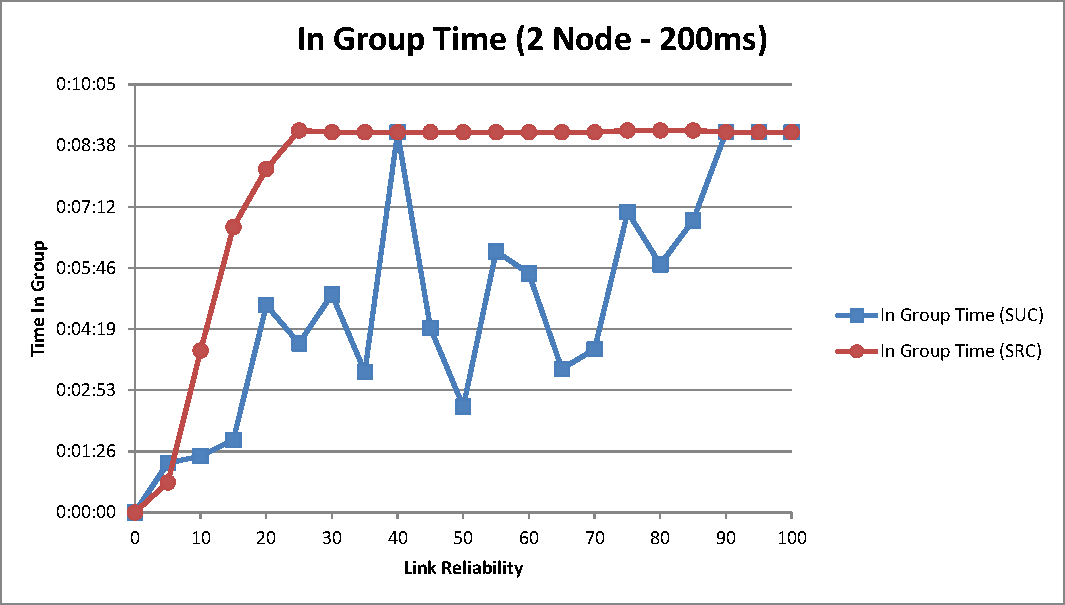
\includegraphics[width=.74\textwidth]{IGT-2NODE-200.pdf}
\caption{Total time spent in group of at least size two for two node system with 200ms resend time}
\label{fig:IGT-2NODE-200}
\end{figure}

\subsection{Test 3 and 4}

Tests 3 and 4 follow the same experimental setup as tests one and two, but the resend time has been reduced to 100ms.
The mean group size is presented in Figure \ref{fig:MGS-2NODE-100}, and the amount of time in group is shown in Figure \ref{fig:IGT-2NODE-100}.

\begin{figure}[!h]
\centering
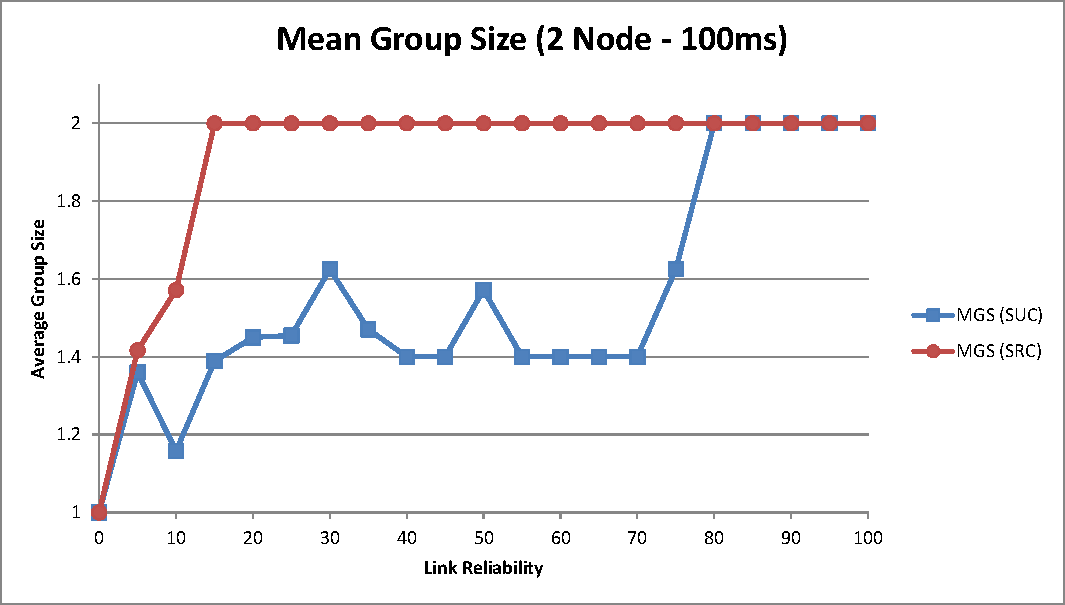
\includegraphics[width=.74\textwidth]{MGS-2NODE-100.pdf}
\caption{Average size of formed groups for two node system with 100ms resend time}
\label{fig:MGS-2NODE-100}
\end{figure}

\begin{figure}[!h]
\centering
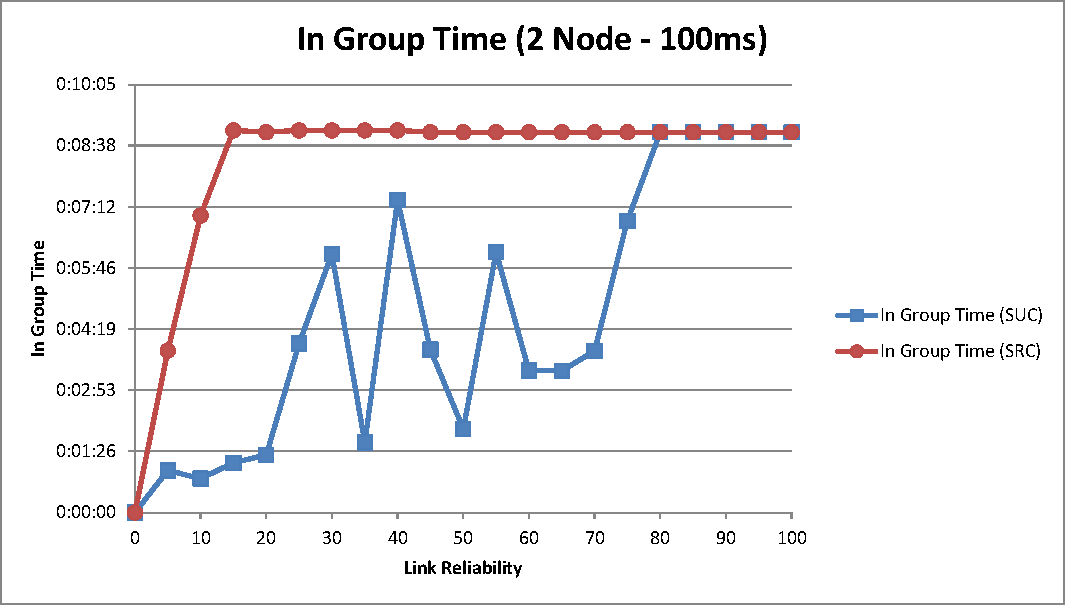
\includegraphics[width=.74\textwidth]{IGT-2NODE-100.pdf}
\caption{Total time spent in group of at least size two for two node system with 100ms resend time}
\label{fig:IGT-2NODE-100}
\end{figure}

\subsection{Test 5 and 6}

Tests five and six are the first to use the transient partition setup. The system is setup with four nodes. Two pairs of nodes are selected. Each pair of nodes can communicate without issue to each other. However, the reliability of the link between the two pairs was varied for each step of the test. These tests used a 200ms resend time. Both SRC and SUC protocols are shown here. As in the previous tests, the window size remained at 8 for the SUC protocol.

\begin{figure}[!h]
\centering
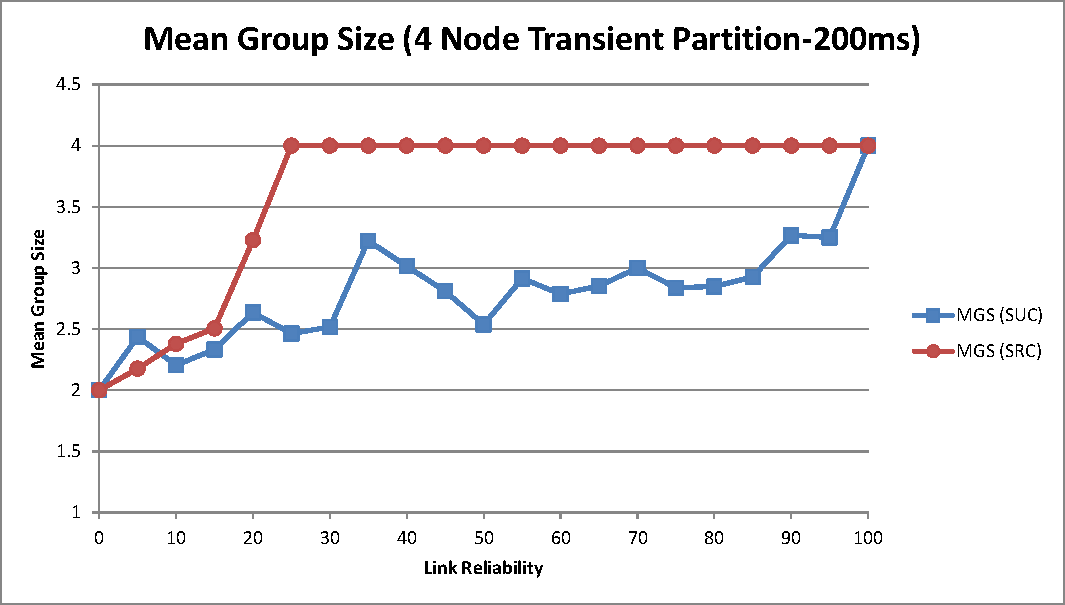
\includegraphics[width=.74\textwidth]{MGS-TRANS-200.pdf}
\caption{Average size of formed groups for a four node system with a transient partition and 200ms resend time}
\label{fig:MGS-TRANS-200}
\end{figure}

\begin{figure}[!h]
\centering
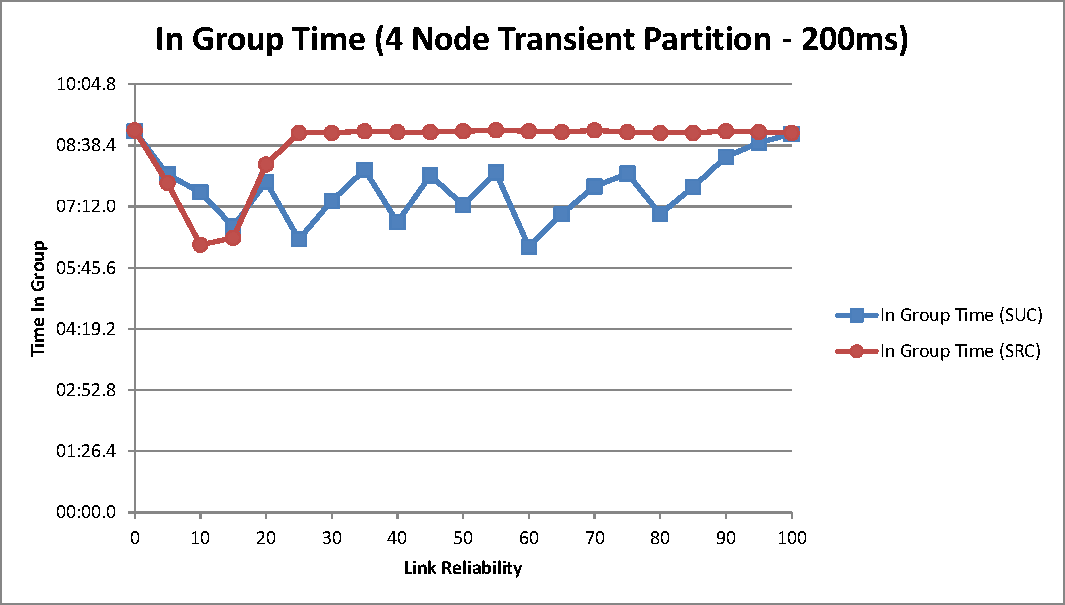
\includegraphics[width=.74\textwidth]{IGT-TRANS-200.pdf}
\caption{Total time spent in group of at least size two for a four node system with a transient partition and 200ms resend time}
\label{fig:IGT-TRANS-200}
\end{figure}

\subsection{Tests 7 and 8}

Tests seven and eight were run with the same setup as Tests 5 and 6, however the resend time was reduced to 100ms.

\begin{figure}[!h]
\centering
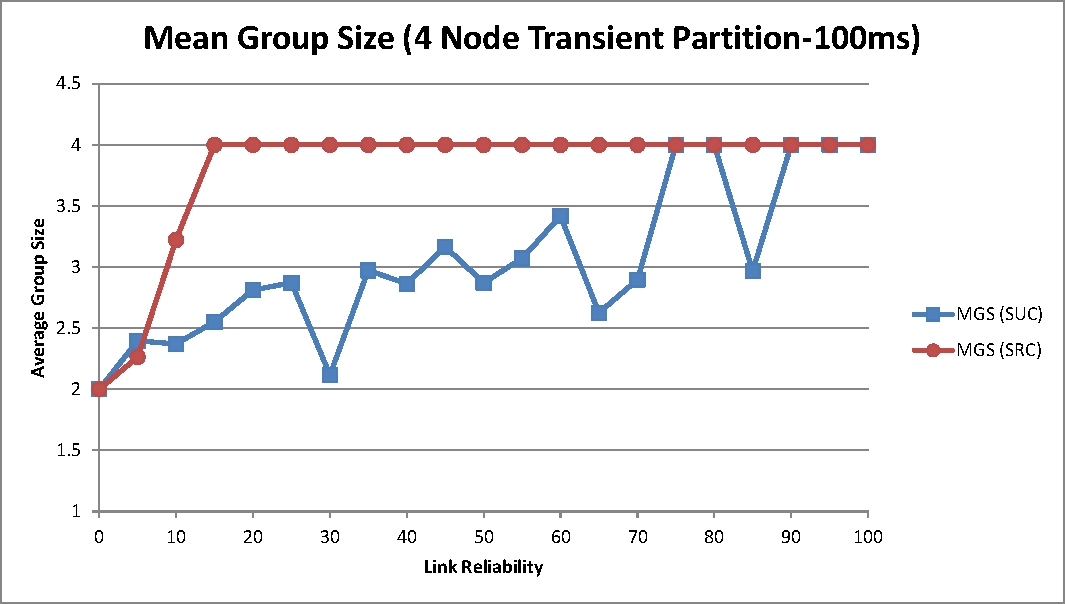
\includegraphics[width=.74\textwidth]{MGS-TRANS-100.pdf}
\caption{Average size of formed groups for a four node system with a transient partition and 100ms resend time}
\label{fig:MGS-TRANS-100}
\end{figure}

\begin{figure}[!h]
\centering
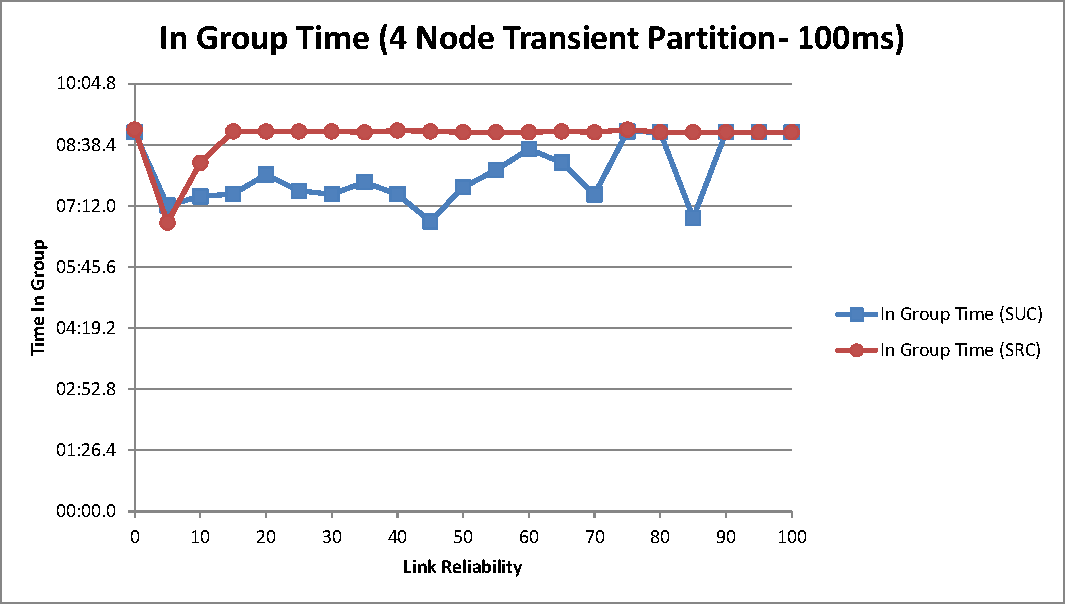
\includegraphics[width=.74\textwidth]{IGT-TRANS-100.pdf}
\caption{Total time spent in group of at least size two for a four node system with a transient partition and 100ms resend time}
\label{fig:IGT-TRANS-100}
\end{figure}

\section{Observations}

As one would expect the mean group size increases  with the stability of the link. This observation can be directly made from the data we collected. However, our measurements often included outliers such as the major one observed in Figure \ref{fig:IGT-TRANS-200}.  To confirm these points as outliers we re-ran the case (Reliability 40 with Test 2, shown in Figures \ref{fig:MGS-2NODE-200} and \ref{fig:IGT-2NODE-200}) multiple times and collected the same measurements. We collected these into Figure \ref{fig:rerun}.

\begin{figure}[!h]
\centering
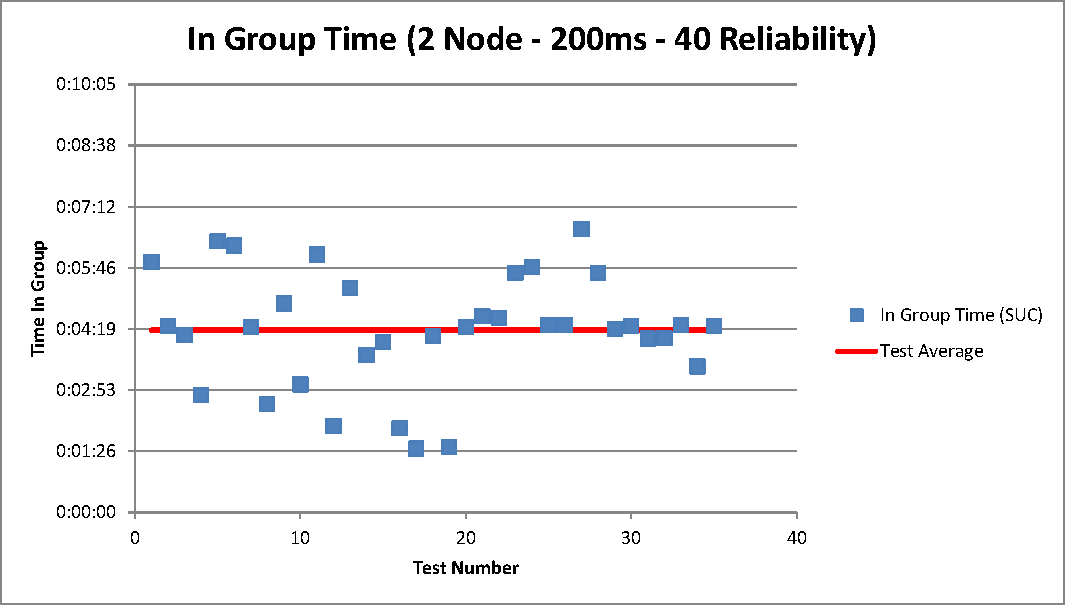
\includegraphics[width=.74\textwidth]{2NODE40RELIABILITY.pdf}
\caption{Total time spent in group of at least size two for the two node node system with the SUC protocol, 200ms resend, and 40 reliability. The average of all points is the solid line}
\label{fig:rerun}
\end{figure}

The points in Figure \ref{fig:rerun} are centered around 4m18s which is where the expected value should be based on the approximate trend of those tests.  Based on further examination, we believe points like these (since they tend to only occur with the SUC protocol) to be cause by two factors. The first factor is that SUC will ignore packets that don't arrive in increasing order, which makes situations where many messages are being passed (such as the election) more difficult to complete. The second factor is the relative stability of the formed group. The timeout for a leader or a member detecting that the other is unreachable is fairly long and given there is a relatively low amount of traffic when it is being delivered,  it is much more likely to arrive and keep the formed group alive. The outlier in Figures \ref{fig:MGS-2NODE-200} and \ref{fig:IGT-2NODE-200} is simply a case where a group formed, and the relative ease of sustaining a group kept it alive for the duration of the test. Other cases can explained similarly.

We had originally selected these two protocols to evaluate their potential in our software. As our development continued we used the SRC protocol as the default (although it is simple to switch between them). The advantages of this are obvious. As presented in nearly every test, even with fairly low link reliability very stable groups formed.  However, it does have limitations: send and wait can be slow. Although it was not relevant in these tests, with a sufficient number of messages in the system, the protocol is not capable of delivering messages fast enough to empty its waiting message queue, even with full reliability.

One of our most noteworthy observations can be made based on our transient partition cases. When the partition completely separates the two nodes, the in group time is at its maximum value.  As the reliability increases however, the transient partition causes the in group time to decrease, since the two sides of the partition are attempting to form groups with each other. This raises questions as to what happens to the underlying physical system when this happens.
\cite{NETWORKTOPOLOGY} showed that sometimes the ideal cyber network does not mimic the physical network. Then however, we have to wonder what happens when the cyber network has link failures or lost messages? Are there circumstances where a group is coordinating using a bus shared with nodes that are not in the same group allows for interactions that destabilize the system?

In the circumstances where the transient link causes an overall decrease in in group time, groups of many different sizes can form. In our case alone, groups of anywhere from one to four members can exist. In a system where coordination is made based on flow contracts \cite{LOADBALANCING}, what issues can arrive when a contract is formed with a node who leaves the group shortly thereafter? Will the effect compound if there are also physical link failures in the system?
